\documentclass[12pt,compress,ngerman,utf8,t,usenames,dvipsnames]{beamer}
\usepackage{etex}
\usepackage[ngerman]{babel}
\usepackage{graphicx}
\usepackage[export]{adjustbox}
\usepackage{multicol}
% \usepackage{animate}
% \usepackage{media9}


\usetheme[numbering=fraction, progressbar=frametitle]{metropolis}


\date{\today}
\institute{University of Freiburg}
\titlegraphic{\vspace{4cm} \hspace{9cm} 
\includegraphics[height=2cm]{Logo-Uni-Freiburg.png}}
\graphicspath{ {../template/} {./images/} }

\title{A Simple Protocol for the Inference of RNA Global Pairwise Alignments}
\author{Felix Karg}

\newif\ifonline
\onlinefalse
% \onlinefalse

\AtBeginSection[]
{
    \large
    \begin{frame}{Content}
        \begin{multicols}{2}
            \tableofcontents[currentsection]
        \end{multicols}
        \clearpage
    \end{frame}
}

\AtBeginSubsection[]
{
    \large
    \begin{frame}{Content}
        \begin{multicols}{2}
            \tableofcontents[currentsection,currentsubsection]
        \end{multicols}
        \clearpage
    \end{frame}
}

% \vspace{0.1cm}



\newcommand{\code}[1]{
    \begin{center}
    \setlength{\fboxrule}{1pt}
    \setlength{\fboxsep}{8pt}
        {\fbox{\parbox{0.81\textwidth}{#1}}}
   \end{center}
}




\begin{document}

\maketitle

% multicols from:
% https://tex.stackexchange.com/questions/24343/splitting-toc-into-two-columns-on-single-frame-in-beamer

%%%%%%%%%%%%%%%%%%%%%%%%%%%%%%%%%%%%%%%%%%%%%%%%%%%%%%%%%%%%%%%%%%%%%%%%%%%%%%%%%%%%%%%%%%%%%%%%%%%%%%%%%%%%%%%%%%%

\begin{frame}{Content}
    \large
    \begin{multicols}{2}
%        \tableofcontents[hidesubsections]
        \tableofcontents[]
    \end{multicols}
    % \clearpage
\end{frame}


% Topics:
%
% Local sequence alignment
% Global and multiple sequence alignment
% Phylogeny (basics)


%%%%%%%%%%%%%%%%%%%%%%%%%%%%%%%%%%%%%%%%%%%%%%%%%%BEGINNING%%%%%%%%%%%%%%%%%%%%%%%%%%%%%%%%%%%%%%%%%%%%%%%%%%%%%%%%
\section{Recap}



\begin{frame}[c]{}
    \center
    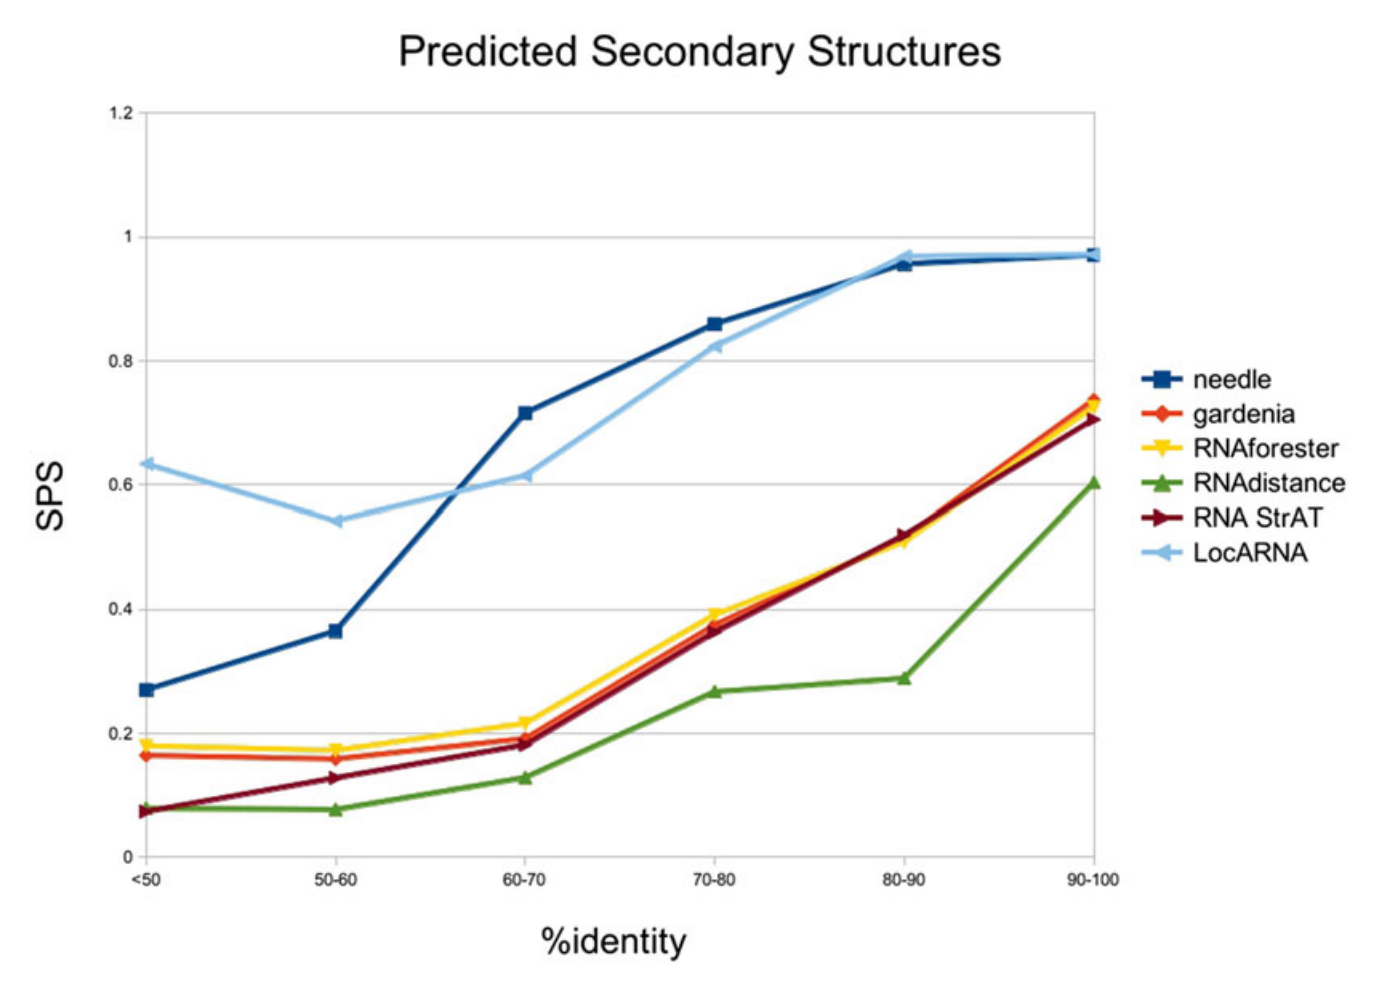
\includegraphics[width=\textwidth]{predicted}
\end{frame}


\begin{frame}[c]{}
    \center
    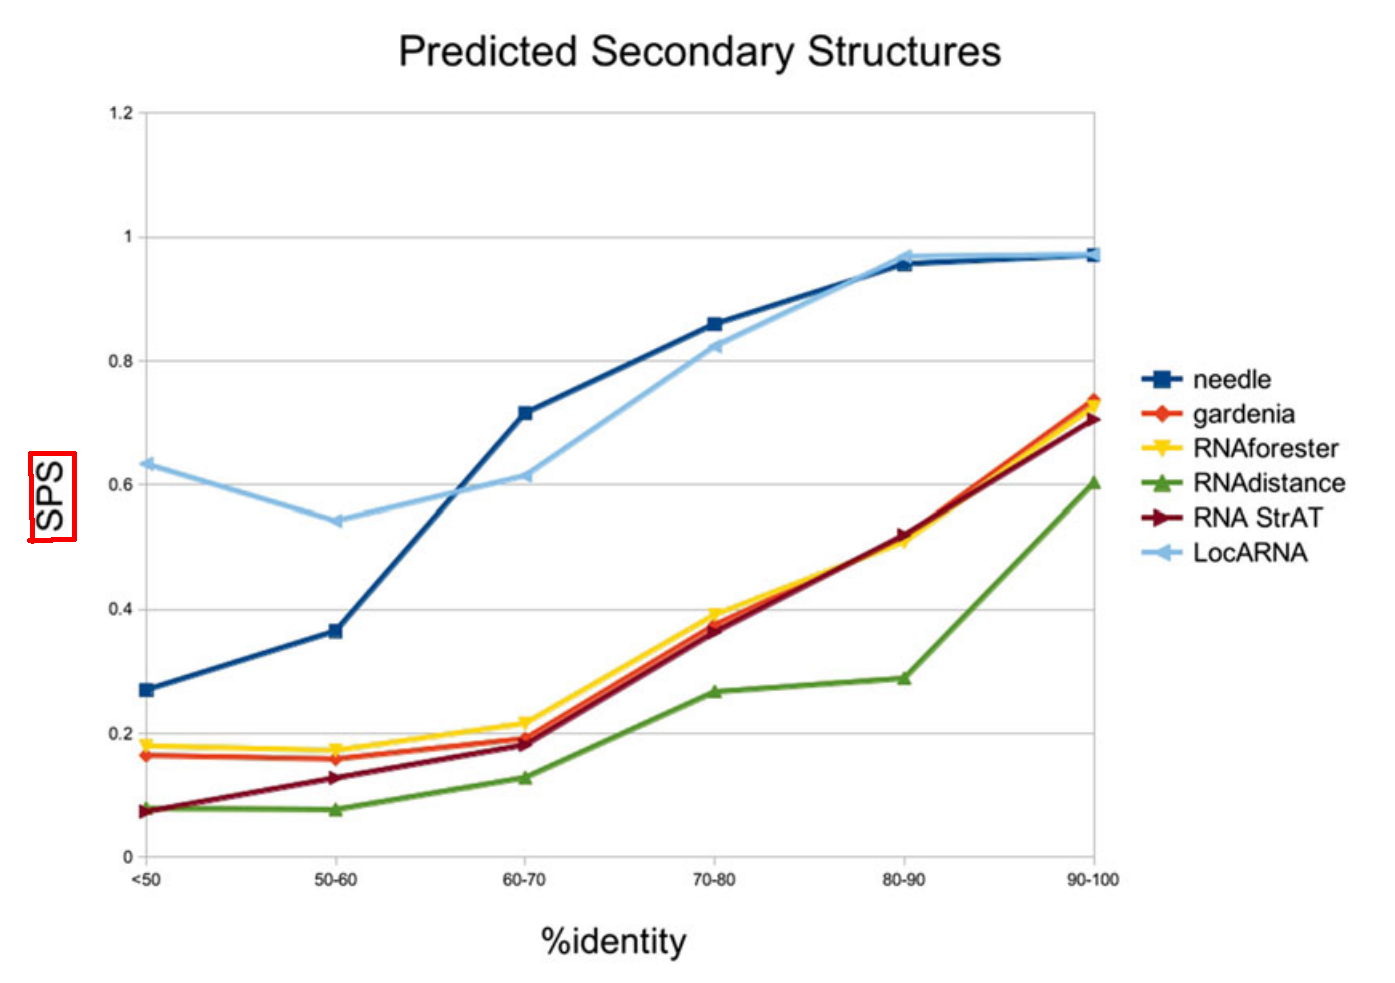
\includegraphics[width=\textwidth]{predicted_sps}
\end{frame}


\begin{frame}[c]{SPS - introduction}
    Sum of Pairs Score
    \newline
%    \vspace{2cm}
    \newline
    \pause
    Used to measure the \only<2-2>{alignment}\only<3->{similiarity} of two RNA sequences
\end{frame}


\begin{frame}[c]{Sequence Similiarity - Example}
    A: \only<4-5>{AAGGC}\only<1-1>{AAGGC}\only<2-3>{{\color{ForestGreen} AAGGC}}\only<1,4->{TT}\only<2-3>{{\color{red}TT}} \\
    B: \only<1-1>{AAGGC}\only<2-5>{{\color{ForestGreen} AAGGC}} \\
    C: \only<1-3>{AAGGC}\only<4->{{\color{ForestGreen} AAGGC}}\only<4-5>{{\color{red}AT}}\only<-3>{AT} \newline
    \newline
    Similiarity: \only<3,5>{60\% = 1 - (2 / 5) } \\
    1 - (edit distance / unaligned length of shorter sequence)
\end{frame}


\begin{frame}[c]{Sequence Similiarity - Example}
    A: {\color{ForestGreen}AAGGC}{\color{red}T}{\color{ForestGreen}T} \\
    B: AAGGC \\
    C: {\color{ForestGreen}AAGGC}{\color{red}A}{\color{ForestGreen}T} \newline
    \newline
    Similiarity: \only<2>{ 86\% = 1 - (1 / 7) } \\
    1 - (edit distance / unaligned length of shorter sequence)
\end{frame}


\begin{frame}[c]{}
    \center
    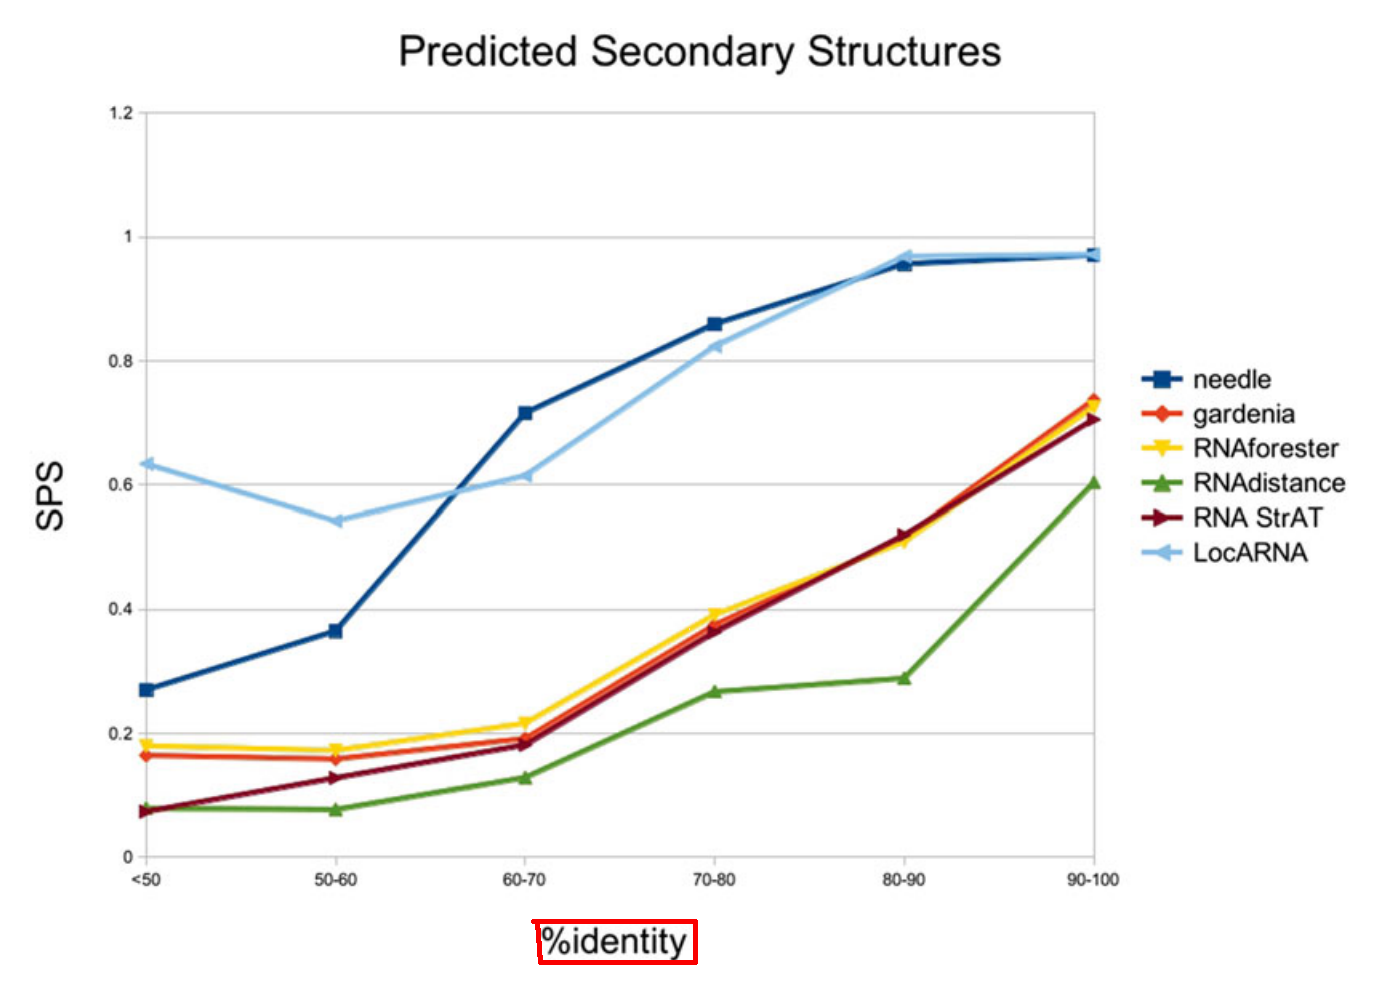
\includegraphics[width=\textwidth]{predicted_identity}
\end{frame}


\begin{frame}[c]{Sequence Identity - Example}
    A: \only<4-5>{AAGGC}\only<1-1>{AAGGC}\only<2-3>{{\color{ForestGreen} AAGGC}}TT \\
    B: \only<1-1>{AAGGC}\only<2-5>{{\color{ForestGreen} AAGGC}} \\
    C: \only<1-3>{AAGGC}\only<4-5>{{\color{ForestGreen} AAGGC}}AT \newline
    \newline
    Identity: \only<3,5>{100\%} \\
    Identical nucleotides / shorter sequence length
\end{frame}


\begin{frame}[c]{Sequence Identity - Example}
    A: {\color{ForestGreen}AAGGC}{\color{red}T}{\color{ForestGreen}T} \\
    B: AAGGC \\
    C: {\color{ForestGreen}AAGGC}{\color{red}A}{\color{ForestGreen}T} \newline
    \newline
    Identity: \only<2>{85\% = 6 / 7} \\
    Identical nucleotides / shorter sequence length
\end{frame}


\begin{frame}[c]{needle}
    \center
    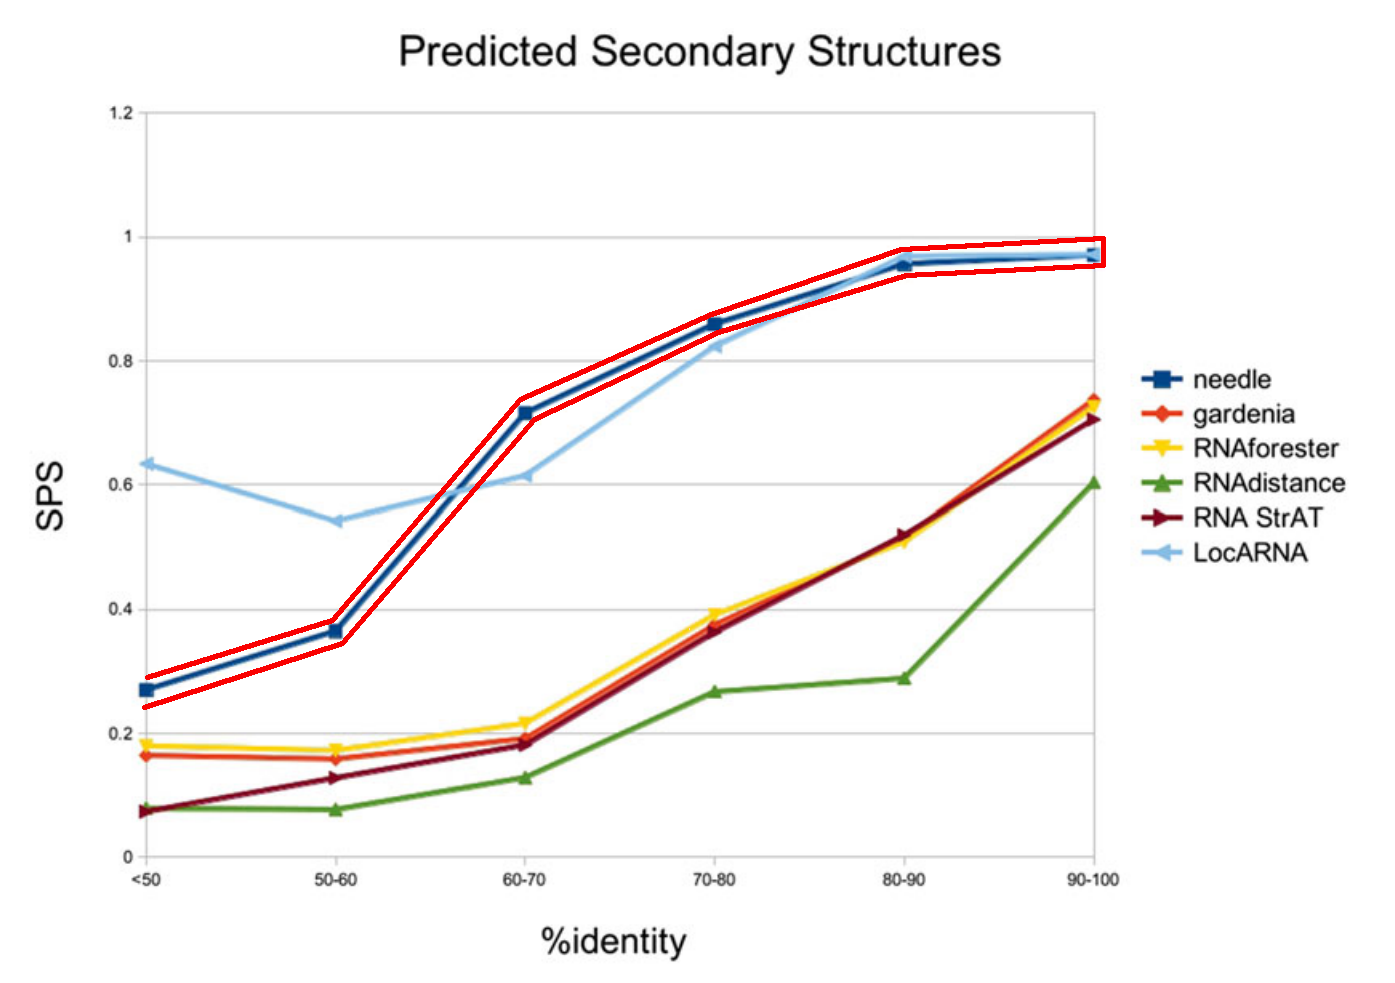
\includegraphics[width=\textwidth]{predicted_needle}
\end{frame}

\begin{frame}[c]{Needleman-Wunsch-Algorithm}
    \center
    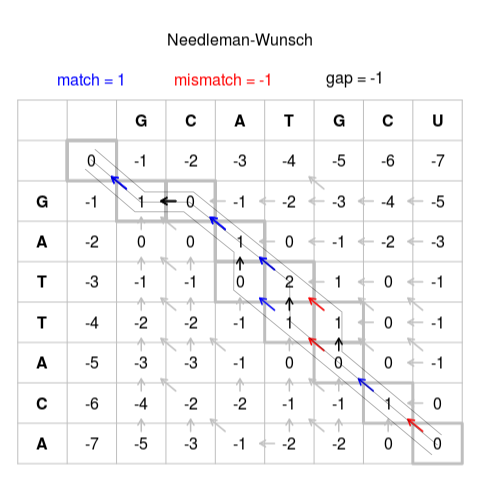
\includegraphics[width=0.75\textwidth]{Needleman-Wunsch_pairwise_sequence_alignment}
\end{frame}













\section{needle}

\begin{frame}[c]{needle - Introduction}
    \begin{itemize}
    \item Sequence based Algorithm \newline
    \pause
    \item part of the EMBOSS package \newline
    \pause
    \item Implementation of the Needleman-Wunsch algorithm
    \end{itemize}
\end{frame}


\begin{frame}[c]{Needleman-Wunsch Algorithm}
    Sometimes also called: \newline
    \begin{itemize}
    \pause
    \item Optimal matching algorithm \newline
    \pause
    \item Global alignment technique
    \end{itemize}
\end{frame}


\section{Sequence Alignment}

\begin{frame}[c]{Sequence Alignment}
    \begin{itemize}
    \item local sequence alignment \newline
    \pause
    \item global sequence alignment \newline
    \pause
    \item glocal sequence alignment
    \end{itemize}
\end{frame}


\begin{frame}[c]{Sequence Alignment - local}
    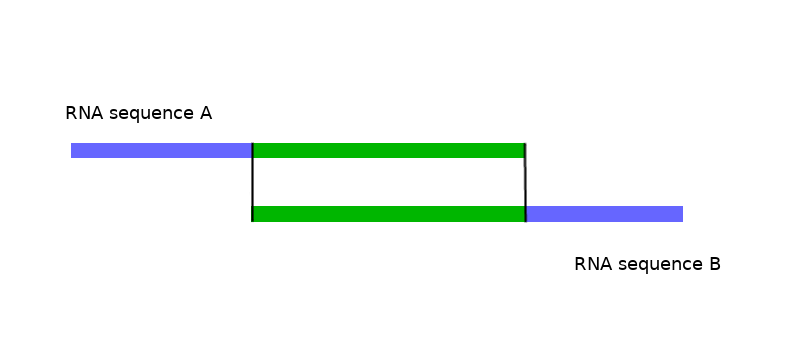
\includegraphics[width=\textwidth]{rna_comparison_local}
\end{frame}

\begin{frame}[c]{Sequence Alignment - global}
    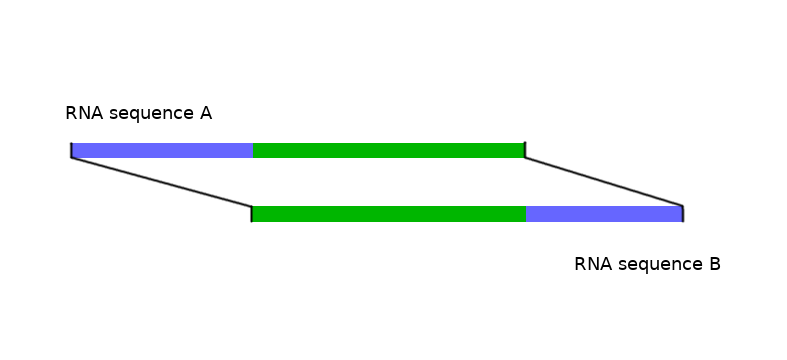
\includegraphics[width=\textwidth]{rna_comparison_global}
\end{frame}

\begin{frame}[c]{Sequence Alignment - glocal}
    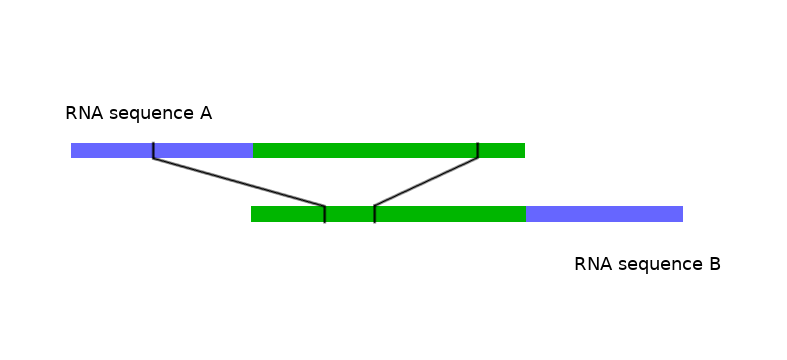
\includegraphics[width=\textwidth]{rna_comparison_glocal2}
\end{frame}


\section{Needleman-Wunsch}


\begin{frame}[c]{Needleman-Wunsch Algorithm - introduction}

    We need a scoring system. \newline \newline
    \pause
    Example: \pause
    \begin{itemize}
    \item Match: 1
    \item Mismatch: -1
    \item Indel: -1
    \end{itemize}

\end{frame}


\begin{frame}[c]{Needleman-Wunsch Algorithm}
    Two sequences to compare: \newline \newline
    \pause
    GCATGCU \newline
    GATTACA
\end{frame}

% tables in latex: https://en.wikibooks.org/wiki/LaTeX/Tables
\begin{frame}[c]{Needleman-Wunsch Algorithm - Example}
    \center
    \begin{tabular}{|c|c|c|c|c|c|c|c|c|}
    \hline
    \phantom{A} & \phantom{A} & \bf{G} & \bf{C} & \bf{A} & \bf{T} & \bf{G} & \bf{C} & \bf{U} \\
    \hline
    \phantom{A} & \onslide<2->{0} & \onslide<3->{-1} & \onslide<3->{-2} & \onslide<3->{-3} & \onslide<3->{-4} & \onslide<3->{-5} & \onslide<3->{-6} & \onslide<3->{-7} \\ \hline
    \bf{G} & \onslide<3->{-1} & \only<4-4>{X} \only<5->{1} & \only<6-6>{X} \only<7->{0} & \only<8->{-1} & \only<8->{-2} & \only<8->{-3} & \only<8->{-4} & \only<8->{-5} \\ \hline
    \bf{A} & \onslide<3->{-2} & \only<6-6>{Y} \only<7->{0} & \only<8->{0} & \only<8->{1} & \only<8->{0} & \only<8->{-1} & \only<8->{-2} & \only<8->{-3} \\ \hline
    \bf{T} & \onslide<3->{-3} & \only<8->{-1} & \only<8->{-1} & \only<8->{0} & \only<8->{2} & \only<8->{1} & \only<8->{0} & \only<8->{-1} \\ \hline
    \bf{T} & \onslide<3->{-4} & \only<8->{-2} & \only<8->{-2} & \only<8->{-1} & \only<8->{1} & \only<8->{1} & \only<8->{0} & \only<8->{-1} \\ \hline
    \bf{A} & \onslide<3->{-5} & \only<8->{-3} & \only<8->{-3} & \only<8->{-1} & \only<8->{0} & \only<8->{0} & \only<8->{0} & \only<8->{-1} \\ \hline
    \bf{C} & \onslide<3->{-6} & \only<8->{-4} & \only<8->{-2} & \only<8->{-2} & \only<8->{-1} & \only<8->{-1} & \only<8->{1} & \only<8->{0} \\ \hline
    \bf{A} & \onslide<3->{-7} & \only<8->{-5} & \only<8->{-3} & \only<8->{-1} & \only<8->{-2} & \only<8->{-2} & \only<8->{0} & \only<8->{0} \\ \hline

    \end{tabular}
    \end{frame}


\begin{frame}[c]{Needleman-Wunsch Algorithm - Best Matches}
    \center
%     % trim = l b r t
%     \includegraphics[width=\textwidth, clip=true, trim = 300mm 370mm 300mm 370mm]{cogbias}
    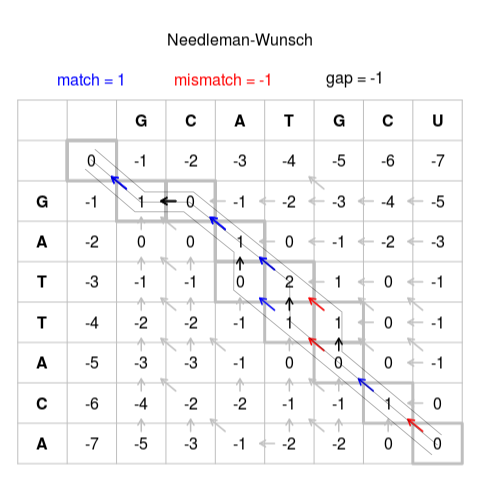
\includegraphics[width=.8\textwidth, clip=true, trim = 0mm 0mm 0mm 25mm]{Needleman-Wunsch_pairwise_sequence_alignment}
\end{frame}


\begin{frame}[c]{Needleman-Wunsch Algorithm - Results}
    \begin{tabular}{l|lll}
    Sequences & \multicolumn{3}{ c }{Best alignments} \\
    \hline
    GCATGCU      & GCATG-CU      & GCA-TGCU      & GCAT-GCU \\
    GATTACA      & G-ATTACA      & G-ATTACA      & G-ATTACA
    \end{tabular}
\end{frame}







% Different Algortihms:
% 
% - sequence-based:
%   - needle
% - folding and aligning
%   - LocARNA
% - Tree-based
%   - gardenia
%   - RNA StrAT
%   - RNAdistance
%   - RNAforester


\section{LocARNA}

\begin{frame}[c]{LocARNA - introduction}
    Two steps:
    \begin{itemize}
    \pause
    \item create base pair probability matrix using RNAfold
    \pause
    \item using these as guide for optimal alignment
    \pause
    \end{itemize}
    (folding and aligning)
\end{frame}


\section{Tree-based sequence alignment}

\subsection{gardenia}

\subsection{RNA StrAT}

\subsection{RNAdistance}

\subsection{RNAforester}



\section{Comparison}

\begin{frame}[c]{Run time Comparison}
    \center
    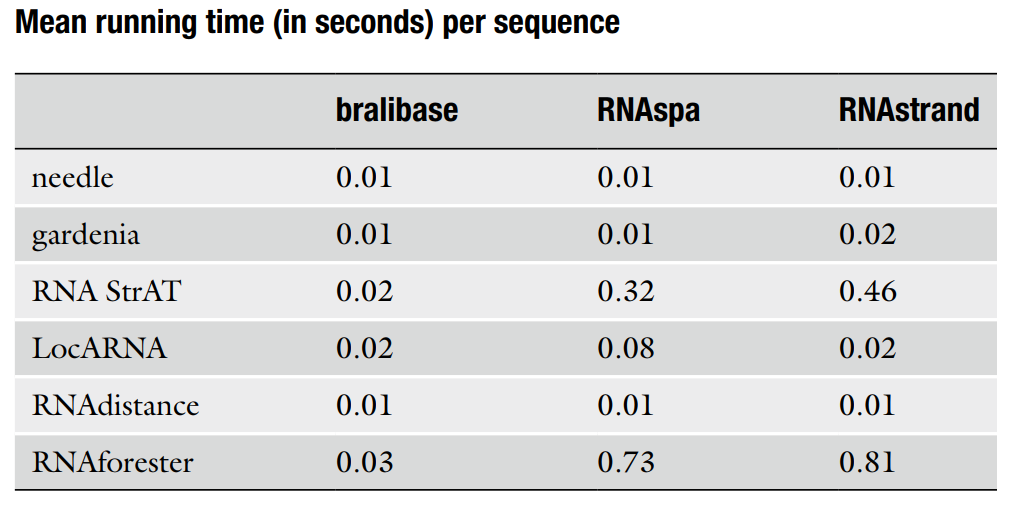
\includegraphics[width=\textwidth]{table}
\end{frame}

\begin{frame}[c]{}
    \center
    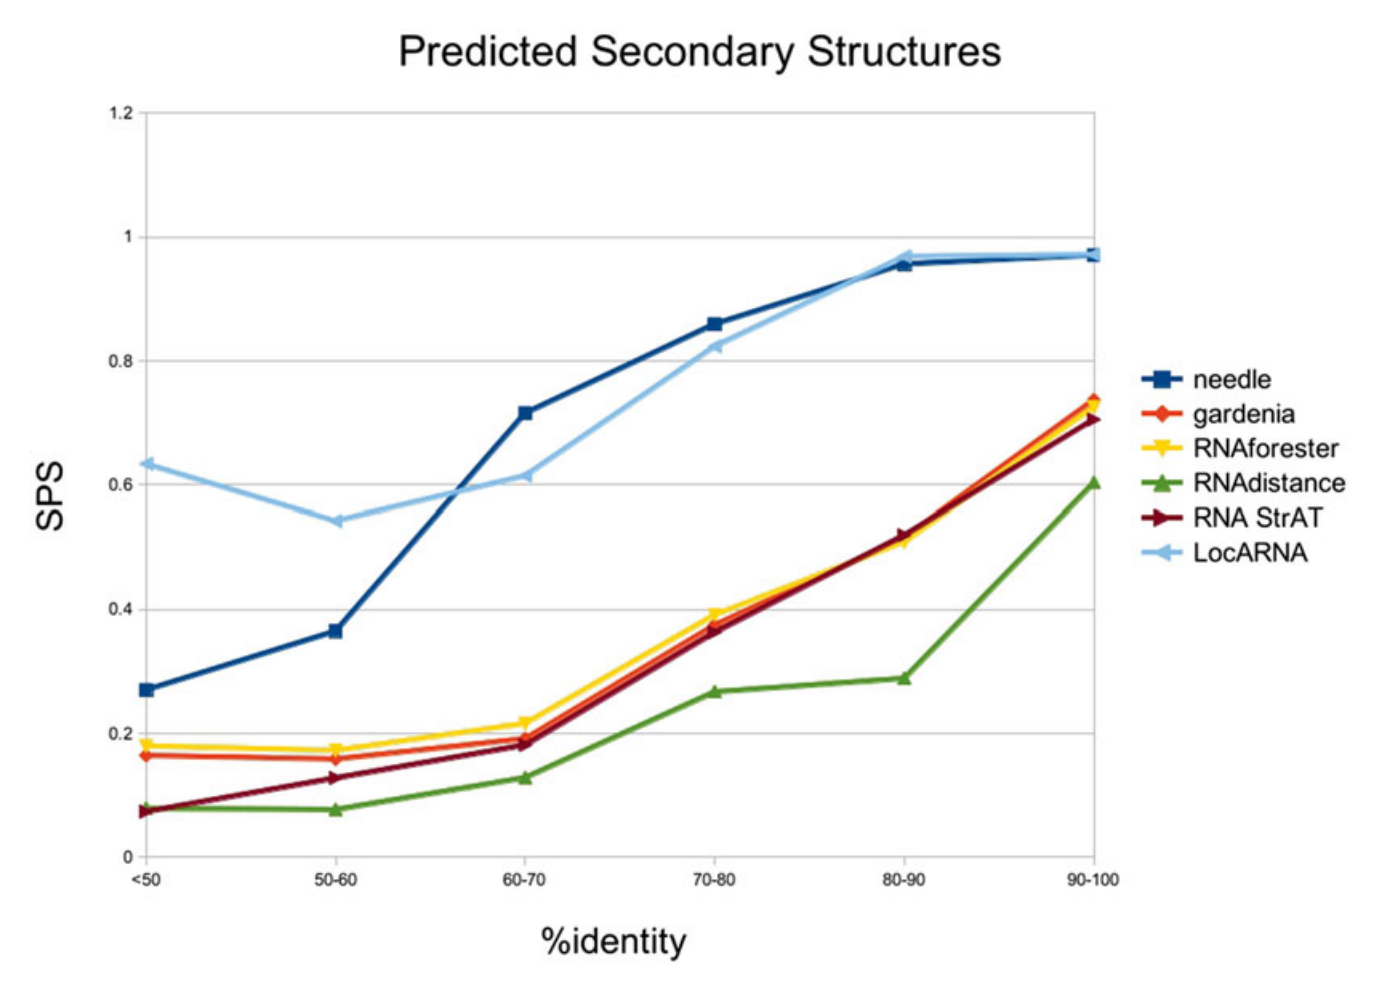
\includegraphics[width=\textwidth]{predicted}
\end{frame}

\begin{frame}[c]{}
    \center
    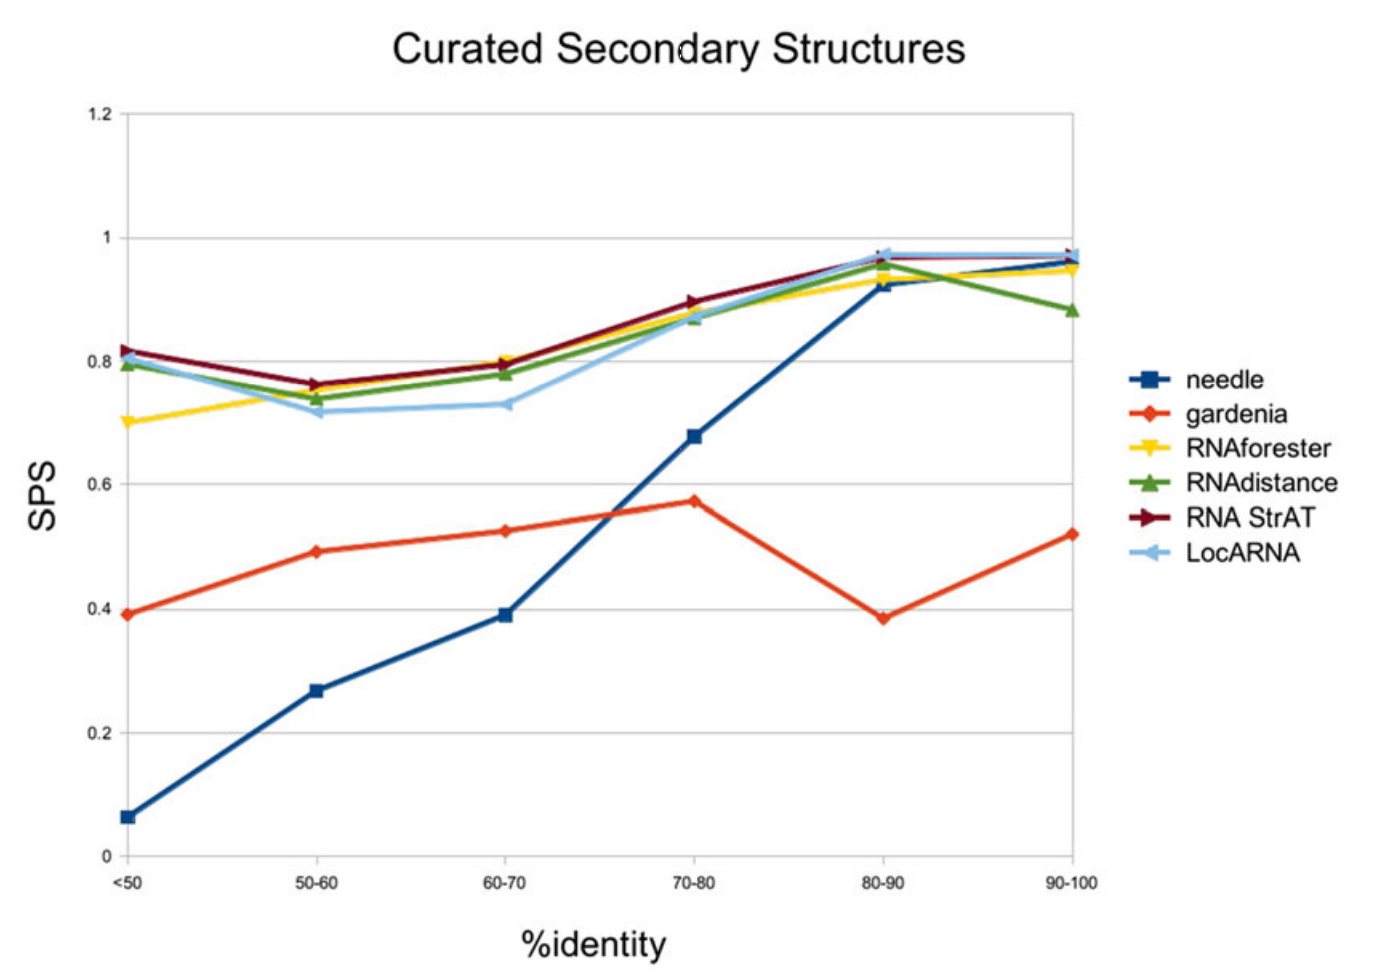
\includegraphics[width=\textwidth]{curated.png}
\end{frame}

\begin{frame}[c]{Proposed Workflow}
    \center
    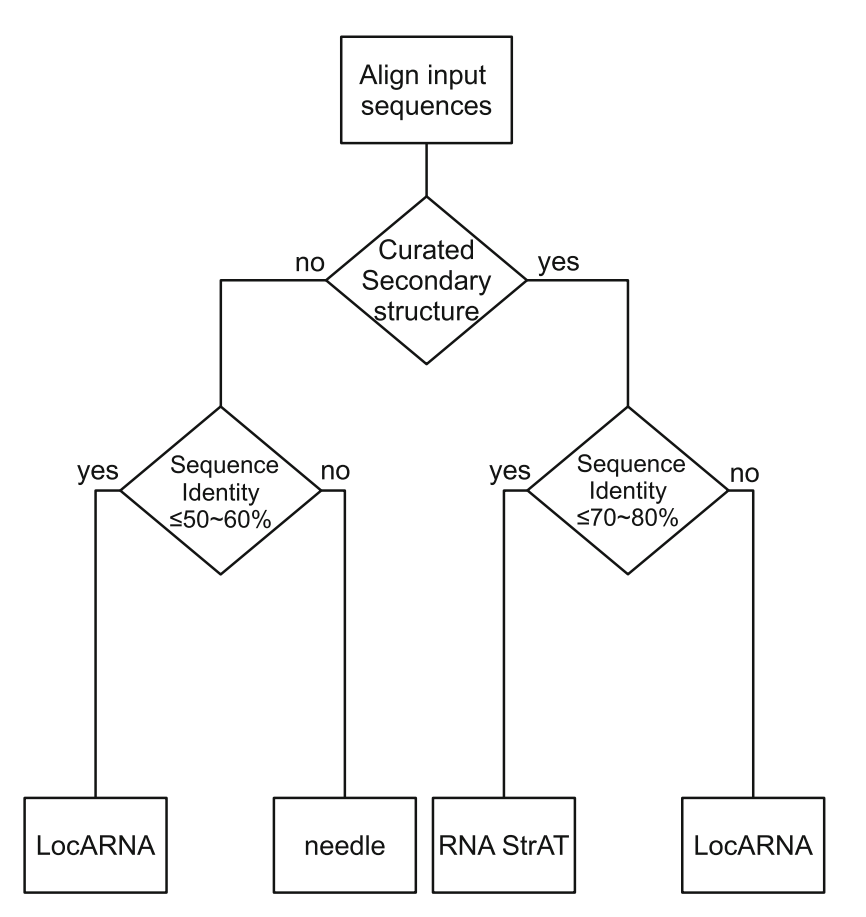
\includegraphics[height=.8\textheight]{flow}
\end{frame}





\section{Sources}

%%%%%%%%%%%%%%%%%%%%%%%%%%CITES%%%%%%%%%%%%%%%%%%%%%%%%%%%%%
\begin{frame}[c,fragile,allowframebreaks]{Sources}
    The slides can be found at: \newline \newline

    \beamertemplatearticlebibitems
    \begin{thebibliography}{10}

    \bibitem{Github}
        {\bf Github}
        \newblock \url{https://github.com/fkarg/things-to-talk-about/tree/master/bioinfII}
    \newline

    \bibitem{Needleman-Wunsch Image}
            {\bf Needleman-Wunsch Image}
            \newblock \url{https://upload.wikimedia.org/wikipedia/commons/3/3f/Needleman-Wunsch_pairwise_sequence_alignment.png}

    \bibitem{Secondary structures Image}
            {\bf Secondary structures Image}
            \newblock \url{https://www.sciencedirect.com/science/article/pii/B9780124200371000014}

    \bibitem{RNA-Bioinformatics Lecture}
            {\bf RNA-Bioinformatics Lecture}
            \newblock \url{https://ilias.uni-freiburg.de/ilias.php?ref_id=1009368&obj\_id=1&cmd=layout&cmdClass=illmpresentationgui&cmdNode=fu&baseClass=ilLMPresentationGUI}


%     \beamertemplatebookbibitems
%     \bibitem{Richard Rumelt}
%         Richard Rumelt
%         \newblock {\em Good Strategy / Bad Strategy}.
%         \newblock The Difference and Why It Matters \\
%                   ISBN: 978-1-78125-154-6
%     \beamertemplatearticlebibitems
%     \bibitem{Lesswrong}
%         Lesswrong
%             \newblock {\em Expecting short Inferential Distances}
%             \newblock \url{http://lesswrong.com/lw/kg/expecting\_short\_inferential\_distances/}
%     \bibitem{Lesswrong}
%         Lesswrong
%             \newblock {\em Cached Thoughts}
%             \newblock \url{http://lesswrong.com/lw/k5/cached\_thoughts/}
%     \bibitem{Zenhabits}
%         Zenhabits
%             \newblock {\em say No so you can say YES}
%             \newblock \url{https://zenhabits.net/say-yes/}
%
%     \bibitem{Wikiquote}
%         Fukuzawa Yukichi
%             \newblock {\em Wikiquote}
%             \newblock \url{https://en.wikiquote.org/wiki/Fukuzawa\_Yukichi}
%
%     \bibitem{SpaceX}
%         SpaceX
%             \newblock {\em SpaceX}
%             \newblock \url{http://www.spacex.com/}
%
%    \bibitem{Wihipedia}
%        Wikipedia
%            \newblock {\em Proton-M}
%            \newblock \url{https://en.wikipedia.org/wiki/Proton-M}
%    \bibitem{Wikipedia}
%        Wikipedia
%            \newblock {\em Ariane 5}
%            \newblock \url{https://en.wikipedia.org/wiki/Ariane\_5}
%    \bibitem{Wikipedia}
%        Wikipedia
%            \newblock {\em Delta IV Heavy}
%            \newblock \url{https://en.wikipedia.org/wiki/Delta\_IV}
   \end{thebibliography}
    % required the allowframebreaks for longer lists

\end{frame}







% \section{Handout}
% \section{Quiz!!!}


% conter deklarieren
\newcounter{official}
\setcounter{official}{\value{page}}

%%%%%%%%%%%%%%%%%%%%%%%%%%%%%%%%%%%%%%%%%%%%%%%%%%%%%%%%%%%%%%%%%%%%%%%%%%%%%%%%%%%%%%%%%%%%%%%%%%%%%%%%%%%%%%%%%%%


\end{document}
